\subsection{Construction of \iotrgen}\label{sec:retrieval}

%\begin{algorithm}[t]
\caption{\iotrgen}\label{alg:iotrgen}
\begin{algorithmic}[1]
\REQUIRE
User \textsf{role}, query $Q$, large language model $\mathcal{M}$, and retrievers $\{\mathcal{R}_i\}_{i=1}^n$.

\ENSURE
Generated answer $A$.

\STATE
\textcolor{gray}{$\triangleright$ \textbf{Procedure of Selector:}}

\STATE
Set prompt $\mathsf{SPT} = (\mathsf{Task}, \mathsf{role}, Q, \{\mathcal{R}_i\}_{i=1}^n)$, where $\mathsf{role}$ includes user's background implicitly and $\mathcal{R}_i$ indicates its description here.
\STATE
Inputting $\mathsf{SPT}$ to $\mathcal{M}$ and get $\{S_i\}_{i=1}^n = \mathcal{M}(\mathsf{SPT})$, where $S_i\in \{\mathsf{True}, \mathsf{False}\}$.

\STATE 
\textcolor{gray}{$\triangleright$ \textbf{Procedure of Self-Querying Retrieval:}}
\FORALL{$i=1, \dots, n$}
\IF{$\mathcal{S}_i = \mathsf{True}$}
\STATE
Execute self-querying retriever $\mathcal{R}_i$ and get documents $D_i=\mathcal{R}_i(Q)$
\ELSE
\STATE
Set $D_i = \mathsf{NULL}$.
\ENDIF
\ENDFOR

\STATE
\textcolor{gray}{$\triangleright$ \textbf{Procedure of Guided Generation:}}

\STATE
Set prompt $\mathsf{UPT} = (\mathsf{Task}, \mathsf{role}, Q, \{\mathcal{D}_i\}_{i=1}^n)$

\RETURN
$A = \mathcal{M}(\mathsf{UPT})$.


\end{algorithmic}
\end{algorithm}

As shown in Figure.~\ref{fig:system}, \iotrgen\ consists of \textit{Adaptive Retrieval} and \textit{Guided Generation}.
We present their detailed constructions as follows.
%The third component utilizes LLM $\mathcal{M}$ to generate the response based on retrieved documents, role, and query, following a straightforward process. 
%This subsection will provide the detailed constructions of the Retriever Selector and Retrievers.

\subsubsection{Adaptive Retrieval}\label{sec:rca}
Recall that we have multiple retrievers, each dedicated to retrieving documents generated from a specific dataset. We achieve adaptive retrieval mechanism works in two aspects: 
\romannumeral1) selecting which retrievers should be activated and \romannumeral2) trying to retrieve only relevant documents while discarding irrelevant ones, even for the activated retrievers.

\smallskip
\noindent \textbf{Design of Selector.}
When user \textsf{role} submits a query $Q$, a straightforward and \textit{static} approach is to $Q$ to all retrievers and gather retrieved documents from them. 
However, this method has the following drawbacks:
\romannumeral1) \textit{Irrelevant Retrievers.} Documents of some retrievers may not be relevant to the query. Retrieving them not only fails to improve the quality of the generated answer but may even negatively affect it.
\romannumeral2) \textit{Resource Costs.} Retrieving unnecessary retrievers leads to increased resource costs, such as computational overhead, during both the retrieval and generation processes.

To address these issues, we introduce an LLM-based adaptive \textit{Selector}. As shown in Figure~\ref{fig:system}, we put the user \textsf{role} with the background, the query $Q$, and the descriptions of all retrievers as \textit{Selector Prompt (SPT)} and input SPT to LLM $\mathcal{M}$, which generates $\{\mathcal{S}_i\}_{i=1}^n$,
where $\mathcal{S}_i = \mathsf{True}$ implies that the retriever $\mathcal{R}_i$ should be activated, and $\mathsf{False}$ indicates not. 
In Table~\ref{tab:selectorexample}, we present the configurations generated by LLaMA3:8B for some example queries submitted by different users.

\iffalse
\iffalse
\begin{table}[]
    \centering
    \caption{The configurations $\{\mathcal{S}_i\}_{i=1}^n$ generated by LLaMA3:8B for different user role and example queries. \ding{52} is for \texttt{True} and \ding{56} is for \texttt{False}.}
    \label{tab:selectorexample}
    \resizebox{0.4\textwidth}{!}{
    \begin{tabular}{@{}c@{\hskip 0.1cm}|
    @{\hskip 0.1cm}>{\centering\arraybackslash}p{4.5cm}@{\hskip 0.1cm}|
    @{\hskip 0.1cm}c
    @{\hskip 0.1cm}c
    @{\hskip 0.1cm}c
    @{\hskip 0.1cm}c
    @{\hskip 0.1cm}c
    @{}}
    \toprule
    \toprule
         Role & Example Query & $\mathcal{S}_1$ & $\mathcal{S}_2$ & $\mathcal{S}_3$ & $\mathcal{S}_4$ & $\mathcal{S}_5$  \\ \midrule
         { \centered{Consumer}} & \centered{ Is it secure to use Signify Smart \\  Lighting in home?} & \ding{52} & \ding{56} & \ding{52} & \ding{56} & \ding{52} \\ \midrule
         {\centered{Security\\ Analyst}} & \centered{ Conduct a security assessment, \\  including vulnerability, exploits, \\  threats, and others, for\\  TP-Link AX6000 Wi-Fi Router.} & \ding{52} & \ding{52} & \ding{52} & \ding{56} & \ding{56} \\ \midrule
         { \centered{Technical\\ Officer}} & \centered{ Check TTPs and security labeling \\  of the company's WiFi Routers, \\  including TP-Link, D-Link, \\  and ASUS in Singapore.} & \ding{52} & \ding{52} & \ding{56} & \ding{52} & \ding{52} \\ \midrule
         { Developer} & \centered{ Develop a security enhancement \\  roadmap for the next generation\\  of TP-Link Wi-Fi routers.} & \ding{52} & \ding{56} & \ding{52} & \ding{56} & \ding{52} \\ \midrule
         { Trainer} & \centered{ Prepare a guide on the importance \\   of cybersecurity labeling for smart \\  locks like the August Smart Lock.} & \ding{52} & \ding{56} & \ding{56} & \ding{56} & \ding{52}  \\
         \bottomrule
         \bottomrule
    \end{tabular}}
\end{table}
\fi 
\fi 

\begin{table}[ht]
    \centering
    \caption{Selector configurations $\{\mathcal{S}_i\}_{i=1}^n$ generated by LLaMA3:8B for different user roles and example queries. \ding{52} indicates \texttt{True} and \ding{56} is for \texttt{False}.}
    \label{tab:selectorexample}
    \resizebox{0.48\textwidth}{!}{
    \begin{tabular}{@{}p{1.5cm}|p{6cm}|c c c c c}
    \toprule
    \toprule
    \multicolumn{1}{c|}{\textbf{Role}} & \multicolumn{1}{c|}{\textbf{Example Query}} & $\mathcal{S}_1$ & $\mathcal{S}_2$ & $\mathcal{S}_3$ & $\mathcal{S}_4$ & $\mathcal{S}_5$  \\ \midrule
    Consumer & Is it secure to use Signify Smart Lighting in home? & \ding{52} & \ding{56} & \ding{52} & \ding{56} & \ding{52} \\ \midrule
    Security Analyst & Conduct a security assessment, including vulnerability, exploits, and threats, for TP-Link AX6000 Wi-Fi Router. & \ding{52} & \ding{52} & \ding{52} & \ding{56} & \ding{56} \\ \midrule
    Technical Officer & Check TTPs and security labeling of the company's WiFi Routers, including TP-Link, D-Link, and ASUS in Singapore. & \ding{52} & \ding{52} & \ding{56} & \ding{52} & \ding{52} \\ \midrule
    Developer & Develop a security enhancement roadmap for the next generation of TP-Link Wi-Fi routers. & \ding{52} & \ding{56} & \ding{52} & \ding{56} & \ding{52} \\ \midrule
    Trainer & Prepare a guide on the importance of cybersecurity labeling for smart locks like the August Smart Lock. & \ding{52} & \ding{56} & \ding{56} & \ding{56} & \ding{52}  \\
    \bottomrule
    \bottomrule
    \end{tabular}
    }
\end{table}



\begin{figure}[h]
    \centering
    \includegraphics[width=0.48\textwidth]{Figures/retriever.pdf}
    \caption{The construction of self-querying retriever based on LangChain and Elastic. When $\mathcal{S}_i=\mathsf{True}$, retrieve documents that are semantically similar to query $Q$ and filtered by metadata.}
    \label{fig:retri}
\end{figure}


\smallskip
\noindent \textbf{Self-Querying Retrievers.}
However, even the activated retrievers may return information that does not meet requirements, \eg, mismatch \textit{id} and \textit{products}. To address this problem, we make use of a self-querying technique to filter documents by \textsf{metadata}. 



\begin{figure*}[h]
    \centering 
\includegraphics[width=\linewidth]{Figures/code3.jpg}
\caption{Metadata fields information and examples for the self-querying retriever corresponding to the VARIoT vulnerabilities dataset.}
\label{fig:variotvulcode}
\end{figure*}


\begin{figure*}
    \centering
    \includegraphics[width=\linewidth]{Figures/code4.jpg}
    \caption{The generated queries and filters for VARIoT vulnerabilities and CLS list for the submitted query "What are the security issues with DLink DCS-942 camera?" by a Security Analyst.}
    \label{fig:querytrans}
\end{figure*}

As illustrated in Figure~\ref{fig:retri}, the self-querying retriever is composed of a Query Constructor, Query Translator, Search Params, and VectorStore.
When the user's query $Q$ is passed to Query Constructor, LLM will generate \textit{internal query language elements} based on pre-defined \textit{metadata\_field information} and \textit{metadata\_examples}.
Query Translator converts these elements into a \textit{structured query} with appropriate filters. 
Finally, the structured query and search parameters are applied to the Vector Store to retrieve documents. 
To specialize the self-querying retriever for IoT security, we take the following steps:
\begin{itemize}
    \item[\textcircled{1}] \textbf{Metadata \& Examples.} We provide the metadata field information and examples from relevant datasets. For instance, in the VARIoT vulnerabilities dataset, fields \textit{id} and \textit{products} are utilized as metadata. The corresponding \textit{metadata\_field\_info} and \textit{examples} are illustrated in Figure~\ref{fig:variotvulcode}, And details for other datasets are available in Appendix~\ref{appendix:metadataother}. This ensures the LLM can gain the necessary IoT security-specific knowledge to generate effective internal query language elements from the user's query.
    
    \item[\textcircled{2}] \textbf{Create Structured Queries.} Based on the above customized internal query language elements, Query Translator can create specific structured queries for each retriever. 
    Figure~\ref{fig:querytrans} shows how to enable the retrieval of VARIoT vulnerabilities and CLS lists that are both semantically similar to the query and appropriately filtered by their respective metadata.
\end{itemize}


%Specifically, given any query $Q$ in natural language, the retriever uses LLM-based to extract filters $F$ from $Q$, generate the structured query $\mathcal{Q}$ from $Q$ and $F$, and finally applies $\mathcal{Q}$ to its underlying VectorStore. 

\begin{figure}[h]
    \centering    
{\footnotesize
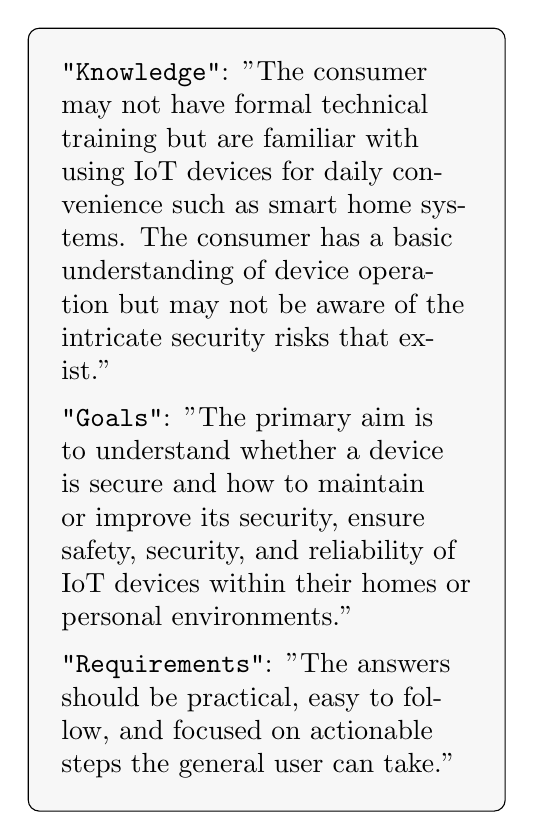
\begin{tikzpicture}
% Draw rounded rectangle with shadow
\node[rectangle, rounded corners, draw=black, fill=black!3!white, text width=0.43\textwidth, inner sep=12pt, align=left] (box) {
\textbf{\texttt{"Knowledge"}}: "The consumer may not have formal technical training but are familiar with using IoT devices for daily convenience such as smart home systems. The consumer has a basic understanding of device operation but may not be aware of the intricate security risks that exist."
\vspace{5pt}\\
\textbf{\texttt{"Goals"}}: "The primary aim is to understand whether a device is secure and how to maintain or improve its security, ensure safety, security, and reliability
of IoT devices within their homes or personal environments."
\vspace{5pt}\\
\textbf{\texttt{"Requirements"}}: "The answers should be practical, easy to follow, and focused on actionable steps the general user can take."
};
\end{tikzpicture}
}
\caption{The background for consumer utilized to guide the \chatiot\ to generate consumer-friendly outputs.}
\label{fig:usecasedef-consumer}
\end{figure}

\subsubsection{Guided Generation}\label{sec:resgen}

After retrieval, one direct step is feeding the retrieved documents and query to LLM to generate the answer. 
However, this simple approach is likely to result in user-unfriendly outputs. 
For example, consumers often lack the expertise needed to fully comprehend highly technical content, making such answers unhelpful and not actionable for them.

To address this issue, we incorporate user-specific backgrounds, including knowledge, goals, and requirements, into each user type's user-friendly prompt template \textit{UPT}. This adjustment guides LLM in generating answers tailored to the user's needs.
The specific background for the general consumer is shown in Figure~\ref{fig:usecasedef-consumer}, demonstrating how we simplify content for easy understanding. The background specifications of other user types can be referred to Appendix~\ref{appendix:bk}.


\begin{algorithm}[t]
\caption{\iotrgen}\label{alg:iotrgen}
\begin{algorithmic}[1]
\REQUIRE
User \textsf{role}, query $Q$, large language model $\mathcal{M}$, and retrievers $\{\mathcal{R}_i\}_{i=1}^n$.

\ENSURE
Generated answer $A$.

\STATE
\textcolor{gray}{$\triangleright$ \textbf{Procedure of Selector:}}

\STATE
Set prompt $\mathsf{SPT} = (\mathsf{Task}, \mathsf{role}, Q, \{\mathcal{R}_i\}_{i=1}^n)$, where $\mathsf{role}$ includes user's background implicitly and $\mathcal{R}_i$ indicates its description here.
\STATE
Inputting $\mathsf{SPT}$ to $\mathcal{M}$ and get $\{S_i\}_{i=1}^n = \mathcal{M}(\mathsf{SPT})$, where $S_i\in \{\mathsf{True}, \mathsf{False}\}$.

\STATE 
\textcolor{gray}{$\triangleright$ \textbf{Procedure of Self-Querying Retrieval:}}
\FORALL{$i=1, \dots, n$}
\IF{$\mathcal{S}_i = \mathsf{True}$}
\STATE
Execute self-querying retriever $\mathcal{R}_i$ and get documents $D_i=\mathcal{R}_i(Q)$
\ELSE
\STATE
Set $D_i = \mathsf{NULL}$.
\ENDIF
\ENDFOR

\STATE
\textcolor{gray}{$\triangleright$ \textbf{Procedure of Guided Generation:}}

\STATE
Set prompt $\mathsf{UPT} = (\mathsf{Task}, \mathsf{role}, Q, \{\mathcal{D}_i\}_{i=1}^n)$

\RETURN
$A = \mathcal{M}(\mathsf{UPT})$.


\end{algorithmic}
\end{algorithm}

Formally, we summarize and show the workflow of \iotrgen\ in algorithm~\ref{alg:iotrgen}.
